\begin{frame}{Model Selection}
    \begin{itemize}
        \item We want models to balance efficacy and size.
        \item In multiple linear regression, \textbf{model selection} refers to "pruning" variables that are less important.
        \item Models that have been optimized in this way are referred to as \textbf{parsimonious}. 
        \begin{itemize}
            \item (Think parsimonious = "frugal".)
        \end{itemize}
        \item The model that includes all possible variables is called the \textbf{full model}. 
    \end{itemize}
\end{frame}

\begin{frame}{Identifying Unhelpful Variables}
    The full model:
    \begin{table}[h]
        \centering
        \begin{tabular}{lcccc}
            \hline
                        & Estimate & Std. Error & t value & Pr($>|t|$) \\
            \hline
            (Intercept) & 26.50  & 1.773 &  14.95 & $<$ 2e-16 \\
            trt     &    -48.20  & 0.159 &-303.71 & $<$ 2e-16 \\
            sexM    &     -0.63  & 0.159 &  -3.99 & 7.23e-05 \\
            age     &      0.02  & 0.012  &  1.29 &  0.197     \\
            weight  &     -0.01  & 0.003 &  -2.45 &  0.015   \\
            sys.bp  &     -0.15  & 0.006 & -27.44 & $<$ 2e-16 \\
            dia.bp  &     -0.11  & 0.010 & -10.84 & $<$ 2e-16 \\
            incomelow  &  -0.23  & 0.227 &  -1.01 &  0.314     \\
            incomemed  &  -0.05 &  0.238 &  -0.19  & 0.848     \\
            ldl.pre    &   0.99  & 0.008 & 126.16 & $<$ 2e-16 \\
            \hline
        \end{tabular}
    \end{table}
    Multiple R-squared:  0.9913,	Adjusted R-squared:  0.9912 
\end{frame}

\begin{frame}{Identifying Unhelpful Variables}
    Removing \texttt{income}:
    \begin{table}[h]
        \centering
        \begin{tabular}{lcccc}
            \hline
                        & Estimate & Std. Error & t value & Pr($>|t|$) \\
            \hline
            (Intercept) & 26.41 & 1.767 & 14.95 & $<$ 2e-16 \\
            trt       &  -48.20 & 0.159 & -303.84 & $<$ 2e-16 \\
            sexM      &   -0.62 & 0.159 & -3.91 & 9.82e-05 \\
            age       &    0.02 & 0.012 &  1.29 &  0.196  \\ 
            weight    &   -0.01 & 0.003 & -2.49 &  0.013 \\ 
            sys.bp    &   -0.15 & 0.006 & -27.62 & $<$ 2e-16 \\
            dia.bp    &   -0.10 & 0.010 & -10.83 & $<$ 2e-16 \\
            ldl.pre   &    0.99 & 0.008 & 126.21 & $<$ 2e-16 \\
            \hline
        \end{tabular}
    \end{table}
    Multiple R-squared:  0.9913,	Adjusted R-squared:  0.9912 
\end{frame}

\begin{frame}{Identifying Unhelpful Variables}
    \begin{itemize}
        \item We find that the models have the same $R^2_{adj}$!
        \item Which one should we choose?
        \item Should we remove more variables?
    \end{itemize}
\end{frame}

\begin{frame}{Identifying Unhelpful Variables}
    What if we remove \texttt{trt}?
    \begin{table}[h]
        \centering
        \begin{tabular}{lcccc}
            \hline
                        & Estimate & Std. Error & t value & Pr($>|t|$) \\
            \hline
            (Intercept) & -22.61 & 17.060 & -1.33 & 0.185    \\ 
            sexM     &    -0.29  & 1.537 & -0.19 & 0.853     \\
            age      &     0.05  & 0.113 &  0.47 & 0.636     \\
            weight   &     0.002  & 0.026 &  0.07 & 0.947     \\
            sys.bp   &    -0.15  & 0.054 & -2.79 & 0.005   \\
            dia.bp   &    -0.08  & 0.094 & -0.86 & 0.389     \\
            ldl.pre  &     1.10  & 0.076 & 14.46 & $<$ 2e-16 \\
            \hline
        \end{tabular}
    \end{table}
    Multiple R-squared:  0.1783,	Adjusted R-squared:  0.1733
\end{frame}

\begin{frame}{Model Selection Strategies}
    We will discuss two common model selection approaches:
    \begin{enumerate}
        \item Forward Selection
        \item Backward Elimination
    \end{enumerate}
    These are referred to as \textbf{step-wise} model selection. 
\end{frame}

\begin{frame}{Backward Elimination}
    \begin{itemize}
        \item \textbf{Backward elimination} starts with the full model.
        \item Variables are removed one-at-a-time until $R^2_{adj}$ stops improving.
        \item At each step, we want to remove the least useful variable.
    \end{itemize}
\end{frame}

\begin{frame}{Example}
    Consider a data set on various loans. We want to predict the interest rate. The available variables are
    \begin{itemize}
        \item \texttt{interest\_rate}: loan interest rate
        \item \texttt{income\_var}: whether income source \& amount verified. Takes values verified, source only, and not.
        \item \texttt{debt\_to\_income}: ratio of debt to income
        \item \texttt{credit\_util}: proportion of credit being utilized
        \item \texttt{bankruptcy}: whether borrower has previous bankruptcy
        \item \texttt{term}: length of loan (months)
        \item \texttt{issued}: month and year loan issued
        \item \texttt{credit\_checks}: number of credit checks in last 12 months
    \end{itemize}
\end{frame}

\begin{frame}{Example: Backward Selection}
    The full model is
    \begin{center}
        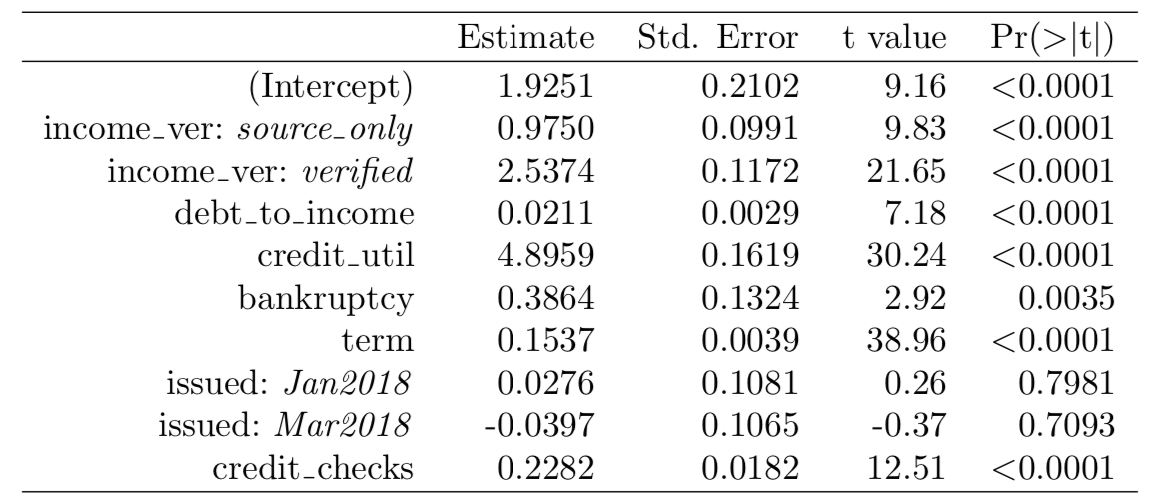
\includegraphics[width=4in]{images/fullmodel.png}
    \end{center}
    There are $n = 10000$ cases in this data set. The variance of the residuals is 18.53, and the variance of the total price is 25.01. \\ Calculate $R^2$ and $R^2_{adj}$.
    %See page 349 bottom for solution
\end{frame}

\begin{frame}{Example: Backward Selection}
    Can we drop a variable and improve $R^2_{adj}$?
    \begin{itemize}
        \item We got a baseline $R^2_{adj}$ on the previous slide.
        \item Variables are eliminated one-at-a-time from the full model.
        \item $R^2_{adj}$ is checked each time.
        \item We move forward with the model with the highest $R^2_{adj}$
    \end{itemize}
    \begin{center}
        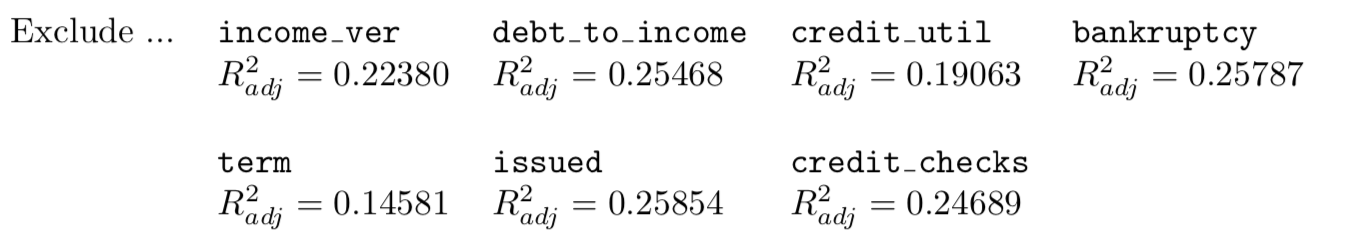
\includegraphics[width=4.7in]{images/back1.png}
    \end{center}
\end{frame}

\begin{frame}{Example: Backward Selection}
    After checking the $R^2_{adj}$ for each potential variable removal, we remove \texttt{issued}.
    \begin{itemize}
        \item Now we repeat the process with the model with \texttt{issued} removed. 
        \item Our new baseline $R^2_{adj}$ is 0.25854.
    \end{itemize}
    \begin{center}
        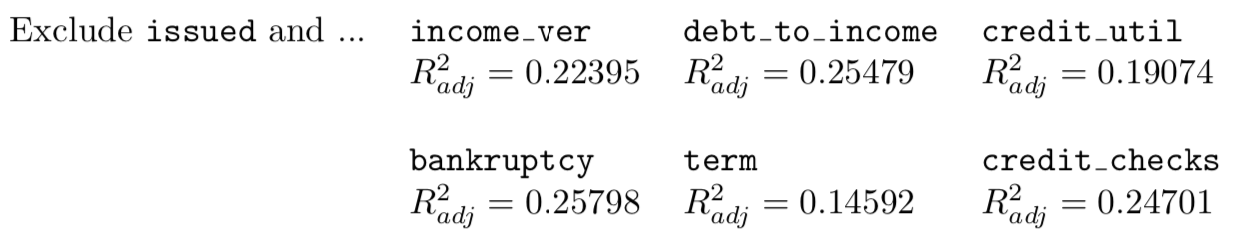
\includegraphics[width=4.5in]{images/back2.png}
    \end{center}
    %We are unable to improve upon the baseline R2adj, so we STOP and do not eliminate any of these predictors.
\end{frame}

\begin{frame}{Example: Backward Selection}
    So our final model is
    \begin{center}
        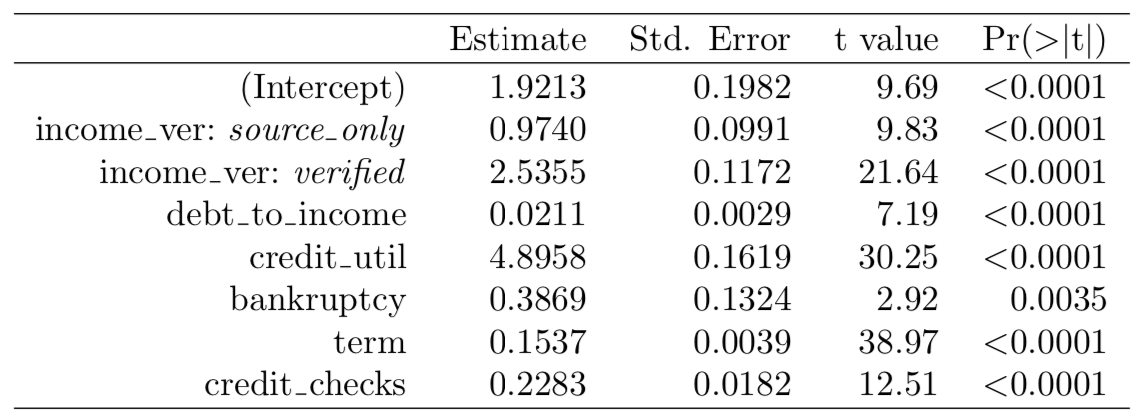
\includegraphics[width=4.7in]{images/finalmodel.png}
    \end{center}
    Write the regression model for these results.
\end{frame}

\begin{frame}{Forward Selection}
    \begin{itemize}
        \item \textbf{Forward selection} is essentially backward selection in reverse.
        \item We start with the model with no variables.
        \item We use $R^2_{adj}$ to add one variable at a time.
        \item We continue to do this until we cannot improve $R^2_{adj}$ any further.
    \end{itemize}
\end{frame}

\begin{frame}{Example: Forward Selection}
    We start with the intercept-only model and (one at a time) examine the model using
    \begin{center}
        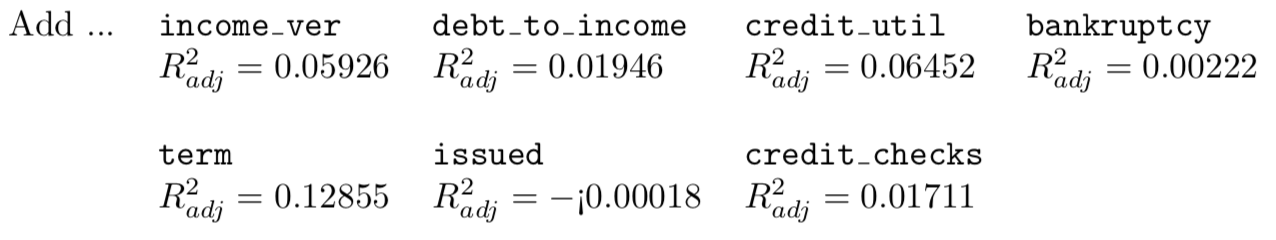
\includegraphics[width=4.5in]{images/forw1.png}
    \end{center}
    to predict interest rate.
    \begin{itemize}
        \item $R^2_{adj}=0$ for the intercept-only model.
    \end{itemize}
\end{frame}

\begin{frame}{Example: Forward Selection}
    \begin{itemize}
        \item We see the biggest improvement with \texttt{term}.
        \item We then check all of the models with \texttt{term} and each other variable.
        \item Our new baseline $R^2_{adj}$ is 0.12855.
    \end{itemize}
    \begin{center}
        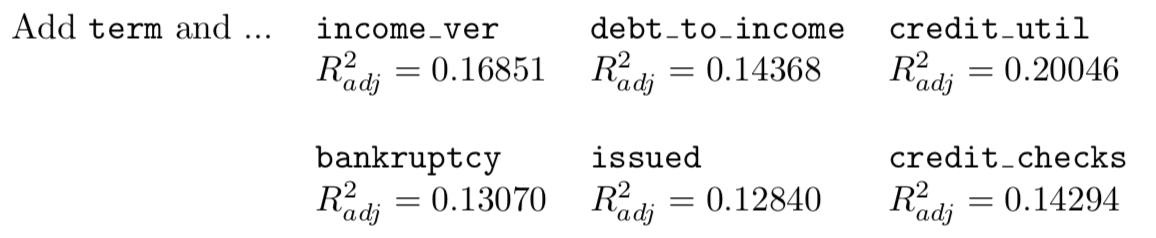
\includegraphics[width=4.5in]{images/forw2.png}
    \end{center}
\end{frame}

\begin{frame}{Example: Forward Selection}
    Moving forward with \texttt{term} and \texttt{credit\_util} (new baseline $R^2_{adj}=0.20046$)
    \begin{center}
        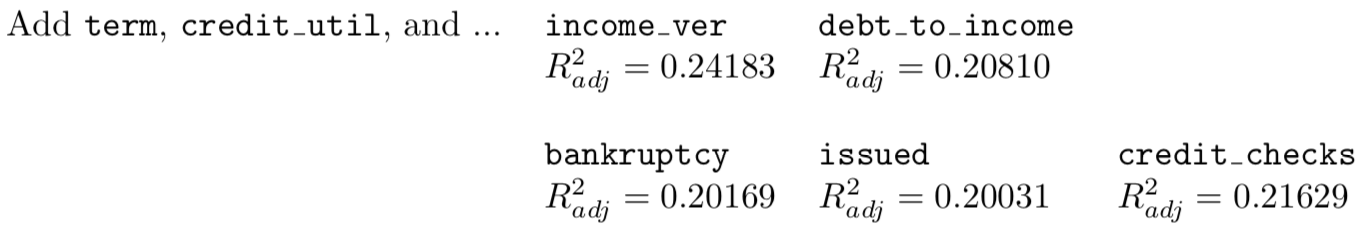
\includegraphics[width=4.5in]{images/forw3.png}
    \end{center}
    So we will include \texttt{income\_var}.
    
    \vspace{12pt}Continuing on, we include \texttt{debt\_to\_income}, then \texttt{credit\_checks}, and \texttt{bankruptcy}.
\end{frame}

\begin{frame}{Example: Forward Selection}
    At this point, we have only \texttt{income} left.
    \begin{itemize}
        \item The current $R^2_{adj}$ is 0.25854.
        \item Including \texttt{income}, we find $R^2_{adj}=0.25843$.
    \end{itemize}
    We conclude with the same model we found in the backward elimination.
    %STOP and do not include income
\end{frame}

\begin{frame}{Model Selection: the P-Value Approach}
    The p-value may be used instead of $R^2_{adj}$. For backward elimination
    \begin{itemize}
        \item Build the full model and find the predictor with the largest p-value.
        \item If the p-value$> \alpha$, remove it and refit the model. 
        \item Repeat with the smaller model.
        \item When all p-values$< \alpha$, STOP. This is your final model.
    \end{itemize}
    Note: it is still important that we remove only one variable at a time!
\end{frame}

\begin{frame}{Model Selection: the P-Value Approach}
    The p-value may be used instead of $R^2_{adj}$. For forward selection
    \begin{itemize}
        \item Fit a model for each possible predictor and identify the model with the smallest p-value.
        \item If that p-value$< \alpha$, add that predictor to the model.
        \item Repeat, building models with the chosen predictor and each additional potential predictor.
        \item When none of the remaining predictors have p-value$<\alpha$, STOP. This is the final model.
    \end{itemize}
    Note: it is still important that we add only one variable at a time!
\end{frame}

\begin{frame}{Model Selection: $R^2_{adj}$ or P-Value?}
    \begin{itemize}
        \item When the primary goal is prediction accuracy, use $R^2_{adj}$.
        \begin{itemize}
            \item This is typically the case in machine learning applications.
        \end{itemize}
        \item When the primary goal is understanding statistical significance, use p-values.
    \end{itemize}
\end{frame}

\begin{frame}{Model Selection: Backward or Forward?}
    \begin{itemize}
        \item Both are perfectly valid approaches.
        \item Statistical software like \texttt{R} can automate either process.
        \item If you have a lot of predictor variables, forward selection may make things easier.
        \begin{itemize}
            \item Note: we can't fit models where $k \ge n$. 
            \item In this setting, forward selection may help us choose which variables to include. 
        \end{itemize}
        \item If you have fewer predictor variables, backward elimination may be easier to use. 
    \end{itemize}
\end{frame}

\begin{frame}{Example: Backward Selection Using P-Values}
    \begin{center}
        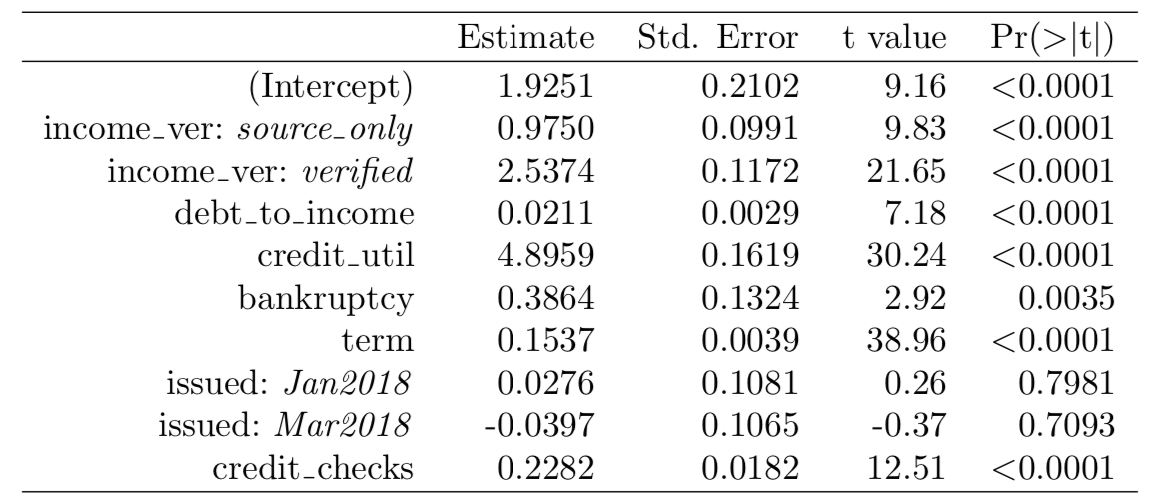
\includegraphics[width=4.7in]{images/fullmodel.png}
    \end{center}
\end{frame}

\begin{frame}{Example: Backward Selection Using P-Values}
    \begin{center}
        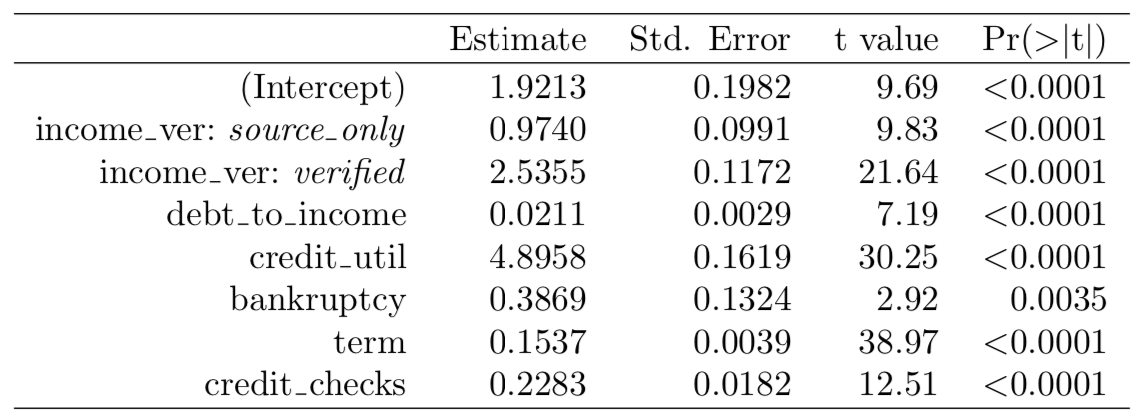
\includegraphics[width=4.7in]{images/finalmodel.png}
    \end{center}
\end{frame}
